\documentclass{article} % A4 paper and 11pt font size
\setcounter{secnumdepth}{0}

\usepackage{amssymb, amsmath, amsfonts}
\usepackage{moreverb}
\usepackage{graphicx}
\newcommand*{\addheight}[2][.5ex]{%
  \raisebox{0pt}[\dimexpr\height+(#1)\relax]{#2}%
}
\usepackage{enumerate}
\usepackage{graphics}
\usepackage[margin=1.25in]{geometry}
\usepackage{color}
\usepackage{tocloft}
\usepackage{subcaption}
\renewcommand{\cftsecleader}{\cftdotfill{\cftdotsep}}
\usepackage{array}
\usepackage{float}
\usepackage{hyperref}
\usepackage{textcomp}
\usepackage[makeroom]{cancel}
\usepackage{bbold}
\usepackage{alltt}
\usepackage{physics}
\usepackage{mathtools}
\usepackage[normalem]{ulem}
\usepackage{amsthm}
\usepackage{tikz}
\usetikzlibrary{positioning}
\usetikzlibrary{arrows}
\usepackage{pgfplots}
\usepackage{bigints}
\allowdisplaybreaks
\pgfplotsset{compat=1.12}

\theoremstyle{plain}
\newtheorem*{theorem*}{Theorem}
\newtheorem{theorem}{Theorem}
\newtheorem*{lemma*}{Lemma}
\newtheorem{lemma}{Lemma}

\makeatletter
\newcommand{\BIGG}{\bBigg@{3}}
\newcommand{\vast}{\bBigg@{4}}
\newcommand{\Vast}{\bBigg@{5}}
\makeatother

\newenvironment{definition}[1][Definition]{\begin{trivlist}
\item[\hskip \labelsep {\bfseries #1}]}{\end{trivlist}}

\newcommand{\E}{\varepsilon}
\def\Rl{\mathbb{R}}
\def\Cx{\mathbb{C}}

\newcommand{\Ei}{\text{Ei}}

\usepackage[T1]{fontenc} % Use 8-bit encoding that has 256 glyphs
\usepackage{fourier} % Use the Adobe Utopia font for the document - comment this line to return to the LaTeX default
\usepackage[english]{babel} % English language/hyphenation

\usepackage{sectsty} % Allows customizing section commands
\allsectionsfont{\centering \normalfont\scshape} % Make all sections centered, the default font and small caps

\usepackage{fancyhdr} % Custom headers and footers
\pagestyle{fancy} % Makes all pages in the document conform to the custom headers and footers
\fancyhead[L]{\bf Sam Fleischer}
\fancyhead[C]{\bf UC Davis \\ Big Data (MAT280)} % No page header - if you want one, create it in the same way as the footers below
\fancyhead[R]{\bf Spring 2016}

\fancyfoot[L]{\bf } % Empty left footer
\fancyfoot[C]{\bf \thepage} % Empty center footer
\fancyfoot[R]{\bf } % Page numbering for right footer
\renewcommand{\headrulewidth}{0pt} % Remove header underlines
\renewcommand{\footrulewidth}{0pt} % Remove footer underlines
\setlength{\headheight}{25pt} % Customize the height of the header

\newcommand{\VEC}[2]{\left\langle #1, #2 \right\rangle}
\newcommand{\ran}{\text{\rm ran }}
\newcommand{\Hilb}{\mathcal{H}}
\newcommand{\lap}{\Delta}

\newcommand{\littleo}[1]{\text{\scriptsize$\mathcal{O}$}\qty(#1)}

\DeclareMathOperator*{\esssup}{\text{ess~sup}}

\newcommand{\problem}[2]{
\vspace{.375cm}
\boxed{\begin{minipage}{\textwidth}
    \section{\bf #1}
    #2
\end{minipage}}
}

\numberwithin{equation}{section} % Number equations within sections (i.e. 1.1, 1.2, 2.1, 2.2 instead of 1, 2, 3, 4)
\numberwithin{figure}{section} % Number figures within sections (i.e. 1.1, 1.2, 2.1, 2.2 instead of 1, 2, 3, 4)
\numberwithin{table}{section} % Number tables within sections (i.e. 1.1, 1.2, 2.1, 2.2 instead of 1, 2, 3, 4)

\setlength\parindent{0pt} % Removes all indentation from paragraphs - comment this line for an assignment with lots of text

\newcommand{\horrule}[1]{\rule{\linewidth}{#1}} % Create horizontal rule command with 1 argument of height

\usepackage{xcolor}
\definecolor{light-gray}{gray}{0.9}

\title{ 
\normalfont \normalsize 
\textsc{UC Davis, Big Data (MAT280), Spring 2016} \\ [25pt] % Your university, school and/or department name(s)
\horrule{2pt} \\[0.4cm] % Thin top horizontal rule
\Huge Homework \#3 \\ % The assignment title
\horrule{2pt} \\[0.5cm] % Thick bottom horizontal rule
}

\author{\huge Sam Fleischer} % Your name

\date{May 16, 2016} % Today's date or a custom date

\begin{document}\thispagestyle{empty}

\maketitle % Print the title

\makeatletter
\@starttoc{toc}
\makeatother

\pagebreak

%%%%%%%%%%%%%%%%%%%%%%%%%%%%%%%%%%%%%%
\problem{Problem 1}{Download the dataset \texttt{crescents.mat} from the Class website and load it into Matlab.  It contains two-hundred points in two dimensions.  If you plot it, you see that the data form two half-moon-like clusters.  Clearly, $k$-means directly applied to this dataset will fail to cluster the data according to these two shapes.  Use the graph Laplacian or diffusion maps (followed by $k$-means) to try to cluster the data as good as possible according to the half-moon shapes.  You can use Matlab's $k$-means function to do the actual clustering once you transformed the data.}
\renewcommand\thefigure{\arabic{figure}}    
\begin{proof}
    Figures 1 and 2 shows the data and the result after spectral clustering. 
    \begin{figure}[ht!]
        \centering
        \begin{minipage}{.5\textwidth}
            \centering
            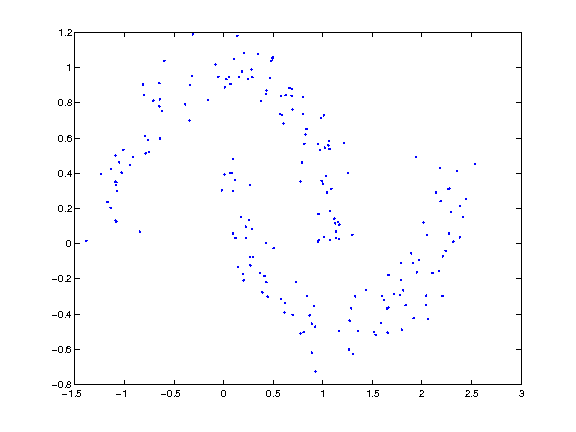
\includegraphics[width=\linewidth]{1.png}
            \captionof{figure}{Original Data}
            \label{fig:1}
        \end{minipage}%
        \begin{minipage}{.5\textwidth}
            \centering
            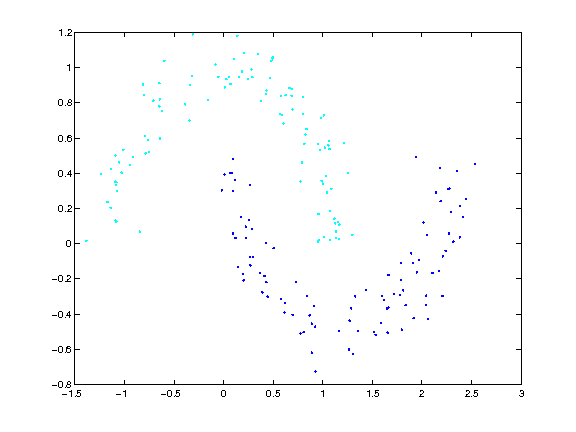
\includegraphics[width=\linewidth]{3.png}
            \captionof{figure}{Data after spectral clustering}
            \label{fig:2}
        \end{minipage}
    \end{figure}
    
    Here are the steps taken to complete this assignment:
    \begin{enumerate}[I.]
        \item
            Define the weight function $w$.
            \begin{align*}
                w_{i,j} = w(p_i, p_j) = \exp[-100\norm{p_i - p_j}_2^2]
            \end{align*}
        \item
            Define the adjacency matrix $A$.
            \begin{align*}
                A_{i,j} = \begin{cases}
                    w_{i,j} & \text{ if } i \neq j \\
                    0 & \text{ if } i = j
                \end{cases}
            \end{align*}
        \item
            Define the graph-Laplacian $L = D - A$ where $D$ is a diagonal matrix with
            \begin{align*}
                D_{i,i} = \sum_{j=1}^n A_{i,j} \qquad \text{ and } \qquad D_{i,j} = 0\ \ \text{ for } i \neq j
            \end{align*}
        \item
            Find the eigenvalues and eigenvectors of $L$ and arrange them in ascending order.  These eigenvalues must necessarily all be non-negative.
        \item
            Define $v_2$ to be the eigenvector corresponding to the second-smallest eigenvalue.  If the $i$\textsuperscript{th} component of $v_2$ is positive, we associate the $i$\textsuperscript{th} data point with the first cluster.  Otherwise, we associate the $i$\textsuperscript{th} data point with the second cluster.
    \end{enumerate}
\end{proof}





%%%%%%%%%%%%%%%%%%%%%%%%%%%%%%%%%%%%%%
\problem{Problem 2}{Download the dataset \texttt{genomedata.mat} from the Class website; it contains Single Nucleid Polymorphisms data from the Human Genome Diversity Project. The data consists of an array consisting of 5000 rows, each row has 1043 different strings.  The 5000 rows are Single Nucleid Polymorphisms, the columns correspond to 1043 different individuals.  The entries are not numerical values (quite annoyingly), but contain the characters `\texttt{AA}', `\texttt{CC}', `\texttt{GG}', `\texttt{TT}', `\texttt{AG}', `\texttt{AC}', `\texttt{TC}', `\texttt{TG}', and (even more annoyingly) also `\texttt{-\hspace{0pt}-}', the latter represents missing measurements.  Your goal is to cluster the data into a small set of clusters.  After loading the file into Matlab, you need to convert the characters into numerical values.  It is up to you which conversion you use (you can use the file \texttt{gen2vec.m} to do the actual conversion, once you have chosen a conversion rule).  Since the data are high-dimensional you first need to reduce the dimension before clustering.  You should attempt the dimension reduction via PCA as well as via diffusion maps.  In both cases you need to decide how many dimensions you want to use.  Also, in both cases you may want to use Matlab's $k$-means function to do the actual clustering after dimension reduction.  Note: Your results may differ from mine, because you will likely choose a different conversion rule.  I did not get a meaningful clustering via PCA, but did achieve reasonable clustering via diffusion maps.}
\begin{proof}
    First, define the following map from $\{\texttt{AA}, \texttt{CC}, \texttt{GG}, \texttt{TT}, \texttt{AG}, \texttt{AC}, \texttt{TG}, \texttt{TC}, \texttt{-\hspace{0pt}-}\}$ to the unit cirtcle (and $0$) in $\Cx$:
    \begin{align*}
        \begin{array}{rcl}
            \texttt{AA} &\mapsto& 1 \\[0.3cm]
            \texttt{TT} &\mapsto& -1 \\[0.3cm]
            \texttt{CC} &\mapsto& i \\[0.3cm]
            \texttt{GG} &\mapsto& -i \\[0.3cm]
            \texttt{AC} &\mapsto& \dfrac{1+i}{\sqrt{2}} \\[0.3cm]
            \texttt{AG} &\mapsto& \dfrac{1-i}{\sqrt{2}} \\[0.3cm]
            \texttt{TC} &\mapsto& \dfrac{-1+i}{\sqrt{2}} \\[0.3cm]
            \texttt{TG} &\mapsto& \dfrac{-1-i}{\sqrt{2}} \\[0.3cm]
            \texttt{-\hspace{0pt}-} &\mapsto& 0
        \end{array}
    \end{align*}
    We choose this map since \texttt{A} never pairs with \texttt{T} and \texttt{C} never pairs with \texttt{G}.  Transform the data given in genomedata.mat in to complex vectors using this map.  We get a $5000\times1043$ matrix of complex numbers, which represents $1043$ data points in $5000$ dimensions.  Next we define the weight function $w$
    \begin{align*}
        w_{i,j} = w(p_i, p_j) = \exp[-\frac{\norm{p_i - p_j}_2^2}{1700}],
    \end{align*}
    and the adjacency matrix $W$
    \begin{align*}
        W_{i,j} = \begin{cases}
            w_{i,j} & \text{ if } i \neq j \\
            0 & \text{ if } i = j.
        \end{cases}
    \end{align*}
    Then define the matrix $M = D^{-1}W$ where $D$ is a diagonal matrix with
    \begin{align*}
        D_{i,i} = \sum_{j=1}^n A_{i,j} \qquad \text{ and } \qquad D_{i,j} = 0\ \ \text{ for } i \neq j.
    \end{align*}
    Next, denote $M_S$ as the normalized matrix $M$:
    \begin{align*}
        M_S = D^{\frac{1}{2}}MD^{-\frac{1}{2}}.
    \end{align*}
    Finally, perform a spectral decomposition of $M_S$ and done it as $M_S = V\Lambda V^T$ where $\Lambda$ is the diagonal matrix containing the eigenvalues of $M_S$ and the columns of $V$ contain the eigenvectors of $M_S$ with respect to their corresponding values in $\Lambda$.  Noting that $M_S$ always has an eigenvalue with norm $1$, we then use MATLAB to find the next four largest (in norm) eigenvalues of $M_S$.  They are:
    \begin{align*}
        \lambda_2 \approx 0.1024963 \qquad \lambda_3 \approx 0.0721643 \qquad \lambda_4 \approx 0.0522477 \qquad \lambda_5 \approx 0.0192484
    \end{align*}
    Note how quickly the eigenvalues decay in Figure (\ref{fig:3}) (this is a $\log$-$\log$ plot).  Only the first few are greater than $10^{-2}$.  We then construct the following diffusion map $U$:
    \begin{align*}
        U = \qty[\begin{array}{cccc}
            \lambda_1^t\phi_1(1) & \lambda_1^t\phi_1(2) & \dots & \lambda_1^t\phi_1(1043) \\
            \lambda_2^t\phi_2(1) & \lambda_2^t\phi_2(2) & \dots & \lambda_2^t\phi_2(1043) \\
            \lambda_3^t\phi_3(1) & \lambda_3^t\phi_3(2) & \dots & \lambda_3^t\phi_3(1043) \\
            \lambda_4^t\phi_4(1) & \lambda_4^t\phi_4(2) & \dots & \lambda_4^t\phi_4(1043) 
        \end{array}]
    \end{align*}
    In order to visualize the relationship of these columns, we compare their magnitudes and arguments in Figure (\ref{fig:4}).
    \begin{figure}[ht!]
        \centering
        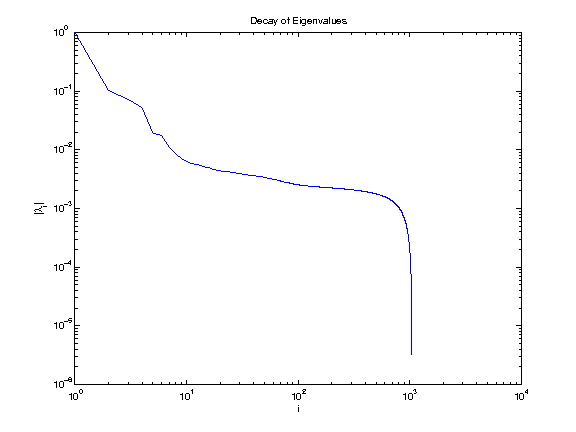
\includegraphics[width=0.75\textwidth]{evals.png}
        \captionof{figure}{Decay of Eigenvalues}
        \label{fig:3}
    \end{figure}
    \begin{figure}
        \centering
        \begin{tabular}[ht!]{ccc}
            \addheight{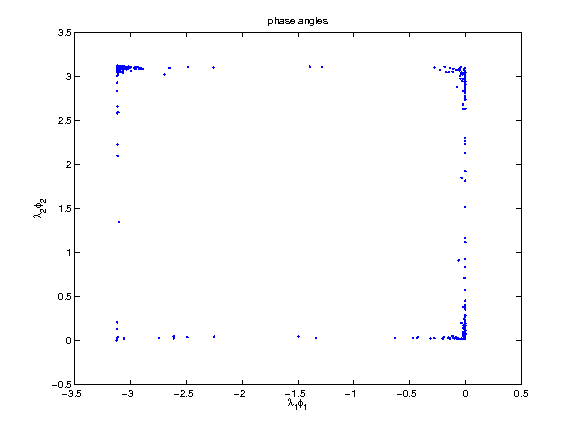
\includegraphics[width=50mm]{12a.png}} & \addheight{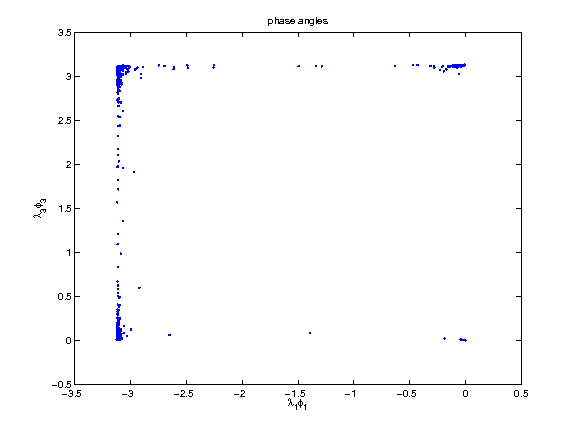
\includegraphics[width=50mm]{13a.png}} & \addheight{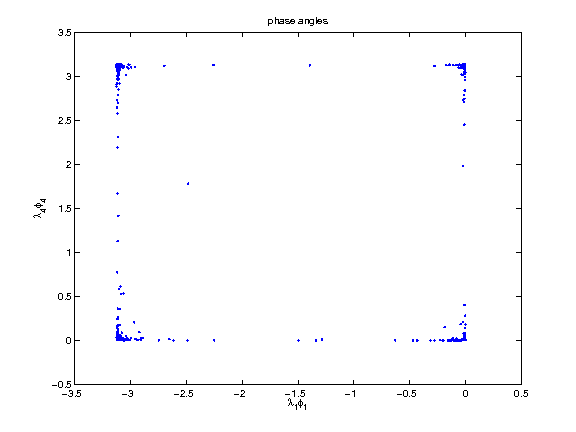
\includegraphics[width=50mm]{14a.png}} \\
            \addheight{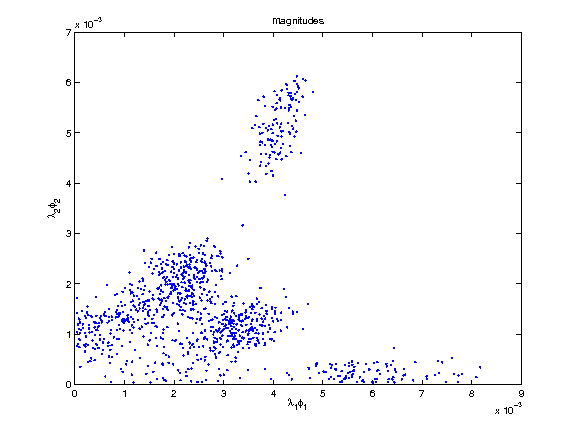
\includegraphics[width=50mm]{12m.png}} & \addheight{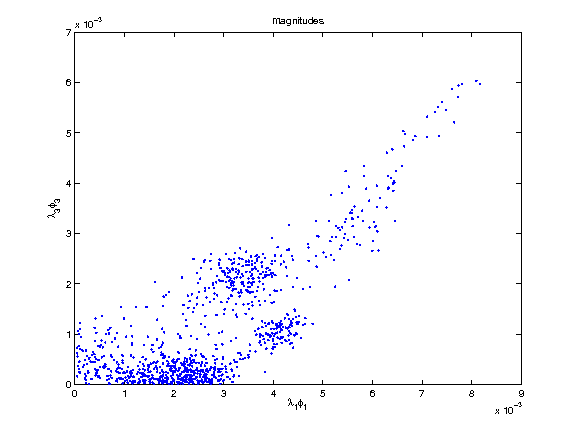
\includegraphics[width=50mm]{13m.png}} & \addheight{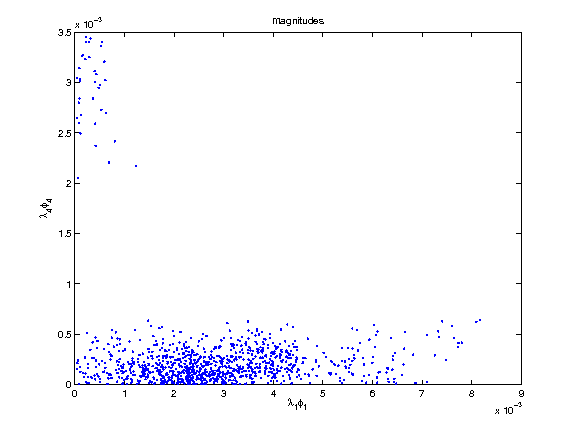
\includegraphics[width=50mm]{14m.png}} \\
            \addheight{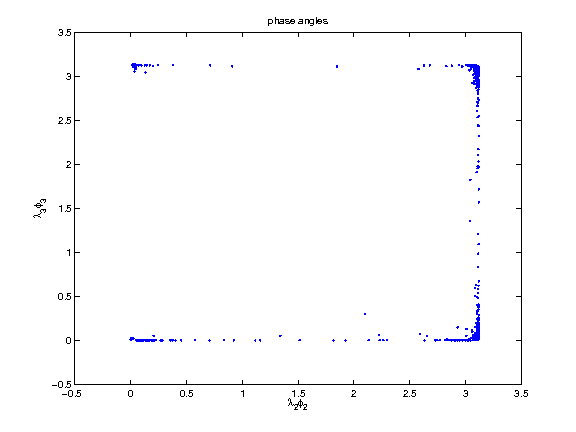
\includegraphics[width=50mm]{23a.png}} & \addheight{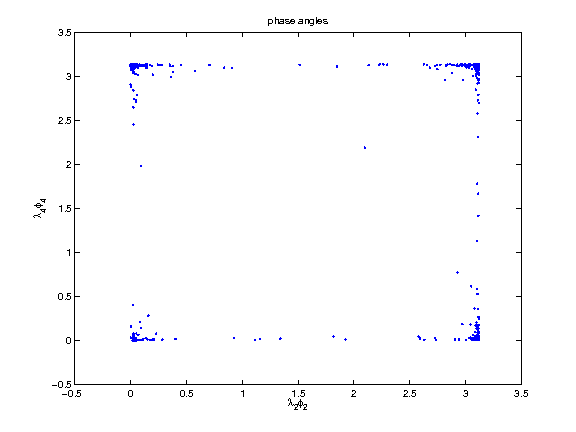
\includegraphics[width=50mm]{24a.png}} & \addheight{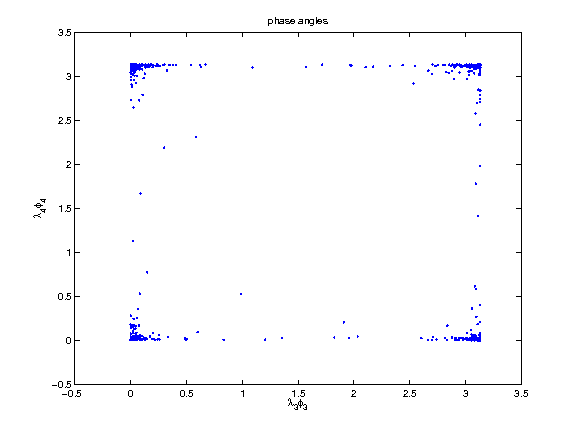
\includegraphics[width=50mm]{34a.png}} \\
            \addheight{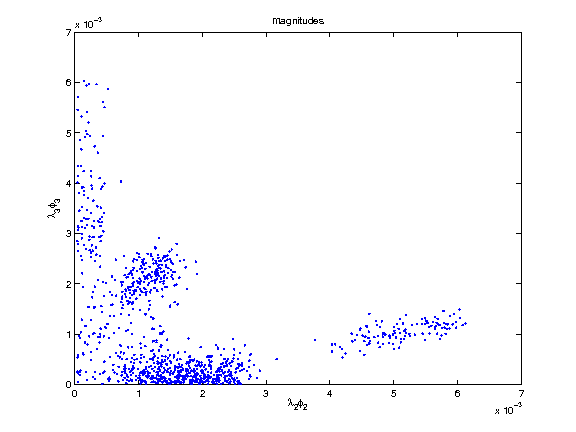
\includegraphics[width=50mm]{23m.png}} & \addheight{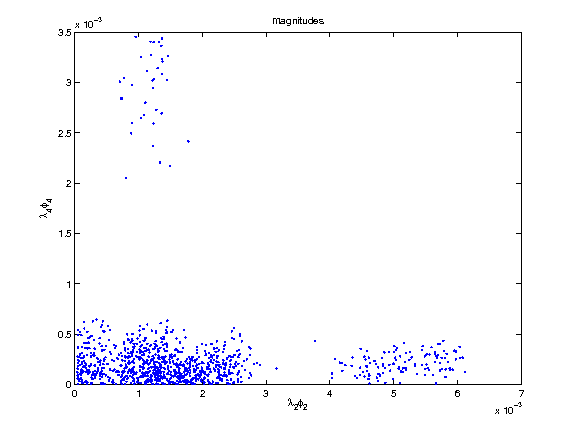
\includegraphics[width=50mm]{24m.png}} & \addheight{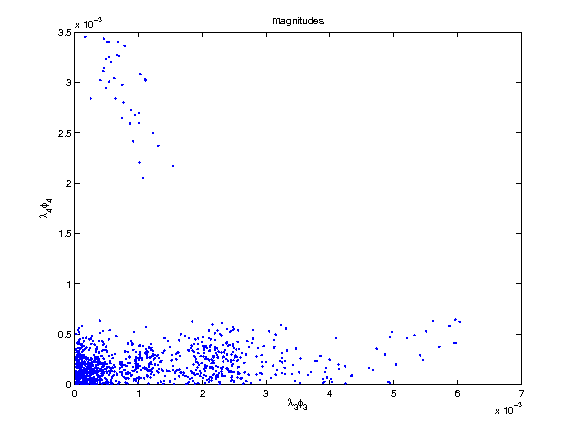
\includegraphics[width=50mm]{34m.png}} \\
        \end{tabular}
        \captionof{figure}{Comparisons of arguments and magnitudes of the columns in $U$.  The top six figures compare column $1$ with columns $2$, $3$, and $4$.  The bottom left four figures compare column $2$ with columns $3$ and $4$, and the bottom right two figures compare column $3$ and column $4$.}
        \label{fig:4}
    \end{figure}
\end{proof}
    






\end{document}
